\section{Echtzeitnachweis}
\subsection{Methoden (skizziert)}
\begin{itemize}
	\item relevante Kenndaten des technischen Prozesses
	\begin{itemize}
		\item Anzahl der unterschiedlichen Anforderungen
		\item Minimale Prozesszeit für jede Anforderung
		\item Minimal zulässige Reaktionszeit $t_{Z_{min}}$ für jede Anforderung
		\item Maximal zulässige Reaktionszeit $t_{Z_{max}}$ für jede Anforderung
		\item Abhängigkeiten zwischen den Ereignissen
	\end{itemize}

	\item maximale Verarbeitungszeit $t_{V_{max}}$ (WCET) für jede Anforderung identifizieren
	
	\item Auslastungsbedingung überprüfen

	\item Rechtzeitigkeitsbedingung verifizieren (Bestimmung von $t_{R_{min}}$ und $t_{R_{max}}$)
\end{itemize}

\subsection{WCET}
\begin{itemize}
	\item Prozesszeiten möglichst kurz
	\item Verarbeitungszeiten möglichst lang 
	\item alle sonstigen Ereignisse im System, die im aktuellen
Prozesszustand möglich sind, treten gleichzeitig (t = 0) auf
\end{itemize}

\subsubsection{Messen}
\begin{itemize}
	\item[+] Sprachunabhängig
	\item[+] meist einfach realisierbar \\
	\item[-] Aussagekraft der Messungen abhängig von vielen Randbedingungen (Prozesszustand, Cache, Schleifen, Verzweigungen)
	\item[-] Theoretisch sämtliche Kombinationen aus Inputdaten erforderlich
(Test-Überdeckung)
	\item[-] Produktiver Code auf Zielplattform oder Simulator erforderlich
	\item[-] Messumgebung/Testrahmen erforderlich
	\item[-] Instrumentierung modifiziert den Code
\end{itemize}

\subsubsection{Analyse}
Aus Quell- oder Zielcode wird ein \underline{Strukturgraph} des Codestücks erstellt
Mit Beschreibung der Zielhardware wird der \underline{längste Pfad} durch den Graphen
gesucht

\subsection{BCET}
Messung wie bei WCET, aber min \underline{geringster Systemlast} und \underline{kürzestem Pfad}

\subsection{maximale Reaktionszeit}
Vorraussetzungen
\begin{itemize}
	\item prioritätengesteuertes Scheduling (Rate Monotonic)
	\item Alle Ergebnisse sind Unabhängig voneinander
\end{itemize}

\subsubsection{Grafisches Verfahren}
\begin{itemize}
	\item \underline{Schnittpunkt mit X-Achse} entspricht Reaktionszeit des \underline{niedrigpriorsten Prozesses}
	\item Für den \underline{nächstniedrigprioren Prozess}: X-Achse um $t_V$ des vorhergehenden Prozesses nach oben verschieben
\end{itemize}

\begin{figure}[h!]
	\begin{center}
		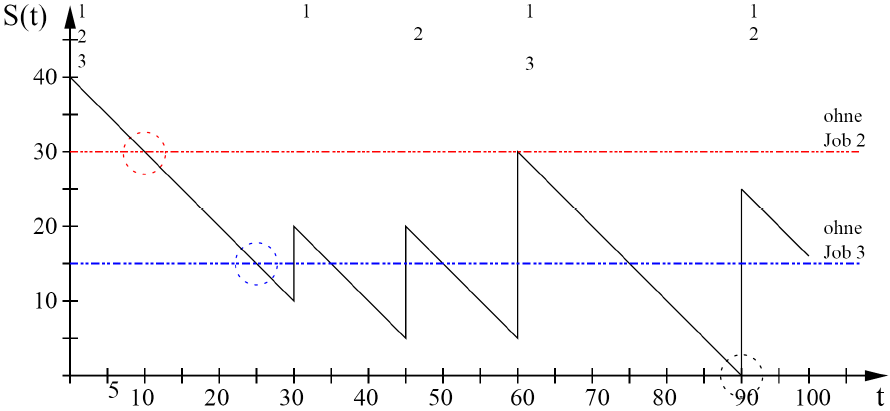
\includegraphics[width=\linewidth]{pics/reaktionszeit}
		\caption{Grafisches Verfahren}
	\end{center}
\end{figure}

\subsection{Schedulingbedingung}
Vorraussetzungen
\begin{itemize}
	\item Scheduling mit statischen Prioritäten (Rate Monotonic...)
	\item Zyklische Tasks ohne Abhängigkeiten
\end{itemize}

\begin{equation*}
	\mu = \sum_{k=1}^{i} \frac{t_{V_k}}{min(t_{Z_{max}}, t_{P_k})} \leq i\cdot (2^{\frac{1}{i}}-1)
\end{equation*}

\begin{tabular}{| c | c |}
	\hline
	i & $\mu$ in \% \\ \hline
	1 & 100 \\
	2 & 82.8 \\
	3 & 78 \\
	4 & 75.7 \\
	5 & 74.3 \\
	10 & 71.8 \\
	$i \rightarrow \infty$ & 69.3 \\ \hline
\end{tabular}